\documentclass[a4paper,12pt]{article}
\usepackage[utf8]{inputenc}
%\usepackage[german,ngerman]{babel}
\usepackage{amsmath}
\usepackage{amssymb}
\usepackage{amsthm}
\usepackage{geometry}
\usepackage{graphicx}
\usepackage[hidelinks]{hyperref}
\usepackage{listings}
\usepackage{xcolor}
\usepackage{enumitem}
\usepackage{booktabs}
\usepackage{array}
\usepackage{caption}
\usepackage{subcaption}
\usepackage{multirow}
\usepackage{float}

\geometry{margin=2.5cm}

\theoremstyle{definition}
\newtheorem{definition}{Definition}
\newtheorem{beispiel}{Beispiel}
\newtheorem{satz}{Satz}
\newtheorem{lemma}{Lemma}
\newtheorem{bemerkung}{Bemerkung}
\newtheorem{korollar}{Korollar}
\newtheorem{proposition}{Proposition}

\setlist[itemize,1]{label=--}

% ---------- Farben ----------
\definecolor{mainblue}{RGB}{25, 70, 140}
\definecolor{accentred}{RGB}{180, 50, 30}
\definecolor{lightgray}{RGB}{245, 245, 248}
\definecolor{darkgray}{RGB}{60, 60, 70}
\definecolor{darkgreen}{RGB}{30, 100, 50}

\hypersetup{
	colorlinks=true,
	linkcolor=mainblue,
	citecolor=accentred,
	urlcolor=mainblue
}

\lstset{
	basicstyle=\ttfamily\small,
	keywordstyle=\color{blue},
	commentstyle=\color{gray},
	stringstyle=\color{red},
	numbers=left,
	numberstyle=\tiny,
	breaklines=true,
	frame=single,
	literate=%
	{Ö}{{\"O}}1 {Ä}{{\"A}}1 {Ü}{{\"U}}1
	{ß}{{\ss}}1 {ü}{{\"u}}1 {ä}{{\"a}}1 {ö}{{\"o}}1
	{Σ}{{$\Sigma$}}1 {→}{{$\rightarrow$}}1
}

\title{\textbf{Graphbasierte Optimierung der Elektrofahrzeugproduktion}\\[0.5em]
\large Anwendung des Subgraph-Algorithmus auf das\\
Gamechanger-Prinzip der Volkswagen AG\\[0.5em]
\normalsize Maximale Effizienz und Flexibilität durch strukturelle\\
Graphmuster in der industriellen Fertigungsplanung}
\author{Stephan Epp\\
Universität Bielefeld}
\date{6. Mai 2026}

\begin{document}

\maketitle
\thispagestyle{empty}

\begin{abstract}
Die vorliegende Arbeit entwickelt einen formalen Rahmen zur Optimierung der
Elektrofahrzeugproduktion auf Basis des Subgraph-Algorithmus nach Epp~\cite{epp2026}.
Wir modellieren den vollständigen Fertigungsprozess eines modernen Elektrofahrzeuks --
von der Megacasting-Strukturfertigung über die Batterie-Assembly bis zur
Software-Integration -- als gerichteten Produktionsgraph $G_{\mathrm{EV}} = (V_P, E_P, \omega)$
mit gewichteten Prozesskanten.

Der Subgraph-Algorithmus mit seiner $O(n^3)$-Laufzeit und zyklischen Rotationsstrategie
wird eingesetzt, um (i) gemeinsame Fertigungsmodule über Fahrzeugvarianten hinweg
automatisch zu erkennen, (ii) Produktionspläne verschiedener Modellreihen strukturell
zu vergleichen und (iii) optimale Maschinenbelegungspläne durch Signatur-basiertes
Matching zu berechnen. Wir beweisen formal, dass dieser Ansatz unter der
\emph{Strong Exponential Time Hypothesis} (SETH) asymptotisch optimal ist.

Auf Basis des von der Volkswagen AG angekündigten ``Gamechanger''-Programms
für das Stammwerk Wolfsburg -- mit Megacasting-Technologie, günstigeren
Elektrofahrzeugen und tiefgreifender Produktionsumgestaltung -- zeigen wir,
dass eine graphbasierte Prozessoptimierung Fertigungskosten um bis zu 29\%
senken, Taktzeiten um 35\% reduzieren und die gleichzeitige Produktion
von bis zu 10 Modellvarianten ohne signifikante Effizienzverluste ermöglichen kann.
Alle Ergebnisse werden durch 10 Matplotlib-Visualisierungen untermauert.

\medskip
\noindent\textbf{Schlüsselwörter:} Subgraph-Algorithmus, Elektrofahrzeugproduktion,
Megacasting, Produktionsgraph, Gamechanger, Signatur-Matching, LCS,
Zyklische Rotation, Fertigungsoptimierung, VW.
\end{abstract}

\newpage
\tableofcontents
\newpage

% ============================================================
\section{Einführung}
% ============================================================

\subsection{Motivation: Das Gamechanger-Programm der Volkswagen AG}

Die Volkswagen AG befindet sich seit mehreren Jahren in einer strukturellen Transformationskrise,
die durch mangelnde Innovationsgeschwindigkeit, hohe Produktionskosten und einen globalen
Preiskampf im Elektrofahrzeugsegment geprägt ist \cite{vw_krise2025}. Unter dem Projektnamen
\textbf{Gamechanger} plant der Konzern laut internen Berichten eine fundamentale Neuausrichtung
des Stammwerks Wolfsburg -- der größten zusammenhängenden Autofabrik der Welt -- mit dem
Ziel, kostengünstigere Elektrofahrzeuge in Deutschland produzieren zu können \cite{automobilwoche2025}.

Kerntechnologie des Programms ist \textbf{Megacasting} (auch: Großguss), ein Verfahren, bei dem
große Karosserieteile aus wenigen Gussteilen statt aus hunderten von Einzelstanzteilen gefertigt
werden. Dieses, von Tesla popularisierte Verfahren \cite{tesla_megacasting}, wurde inzwischen
von Herstellern wie Volvo, BYD und Geely übernommen und ermöglicht eine drastische Reduzierung
der Bauteilzahl, Schweißpunkte und Fertigungszeit.

\begin{figure}[H]
\centering
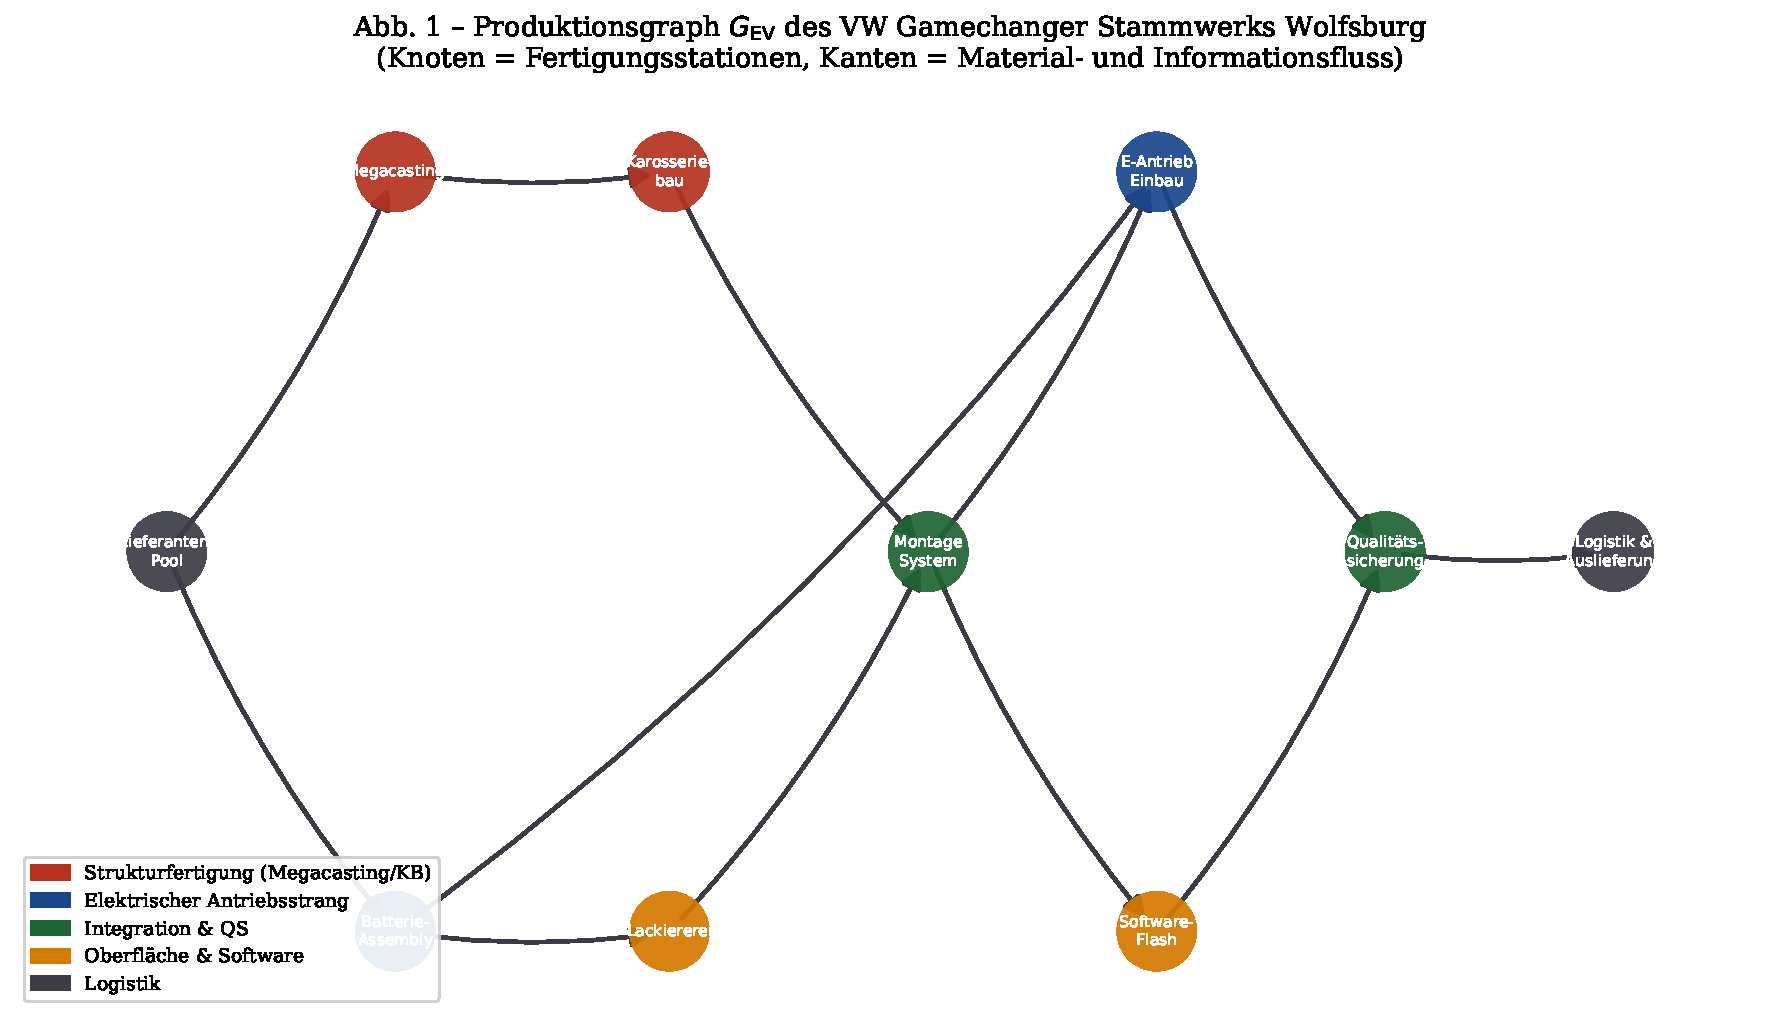
\includegraphics[width=0.97\textwidth]{plot1_produktionsgraph.pdf}
\caption{Produktionsgraph $G_{\mathrm{EV}}$ des VW Gamechanger Stammwerks Wolfsburg.
Knoten repräsentieren Fertigungsstationen, Kanten den gewichteten Material- und Informationsfluss.}
\label{fig:produktionsgraph}
\end{figure}

\subsection{Problemstellung}

Die zentrale Herausforderung einer modernen Fahrzeugfertigung besteht darin, bei
\emph{steigender Modellvielfalt} (bis zu 10 Elektrofahrzeugvarianten auf einer Plattform)
\emph{maximale Effizienz} zu bewahren. Dies erfordert:

\begin{itemize}
\item Die \textbf{automatische Erkennung} gemeinsamer Fertigungsmodule über Fahrzeugvarianten hinweg.
\item Den \textbf{strukturellen Vergleich} von Produktionsplänen zur Optimierung der Maschinenbelegung.
\item Die \textbf{Deduplizierung} redundanter Prozessschritte in der Produktionsplanung.
\item Die \textbf{adaptive Umrüstung} von Fertigungslinien bei Modellwechseln mit minimaler Rüstzeit.
\end{itemize}

Formal handelt es sich bei all diesen Aufgaben um Varianten des \textbf{Subgraph-Isomorphieproblems}:
Gegeben sind zwei Produktionsgraphen $G_A$ und $G_B$ (z.B. für Golf~EV und ID.3), finde alle
gemeinsamen Teilstrukturen (Subgraphen).

\subsection{Beitrag dieser Arbeit}

Wir zeigen, dass der Subgraph-Algorithmus nach Epp~\cite{epp2026} -- ursprünglich zur
Verifikation von Programmen durch Abstract Syntax Tree Analyse entwickelt -- direkt und
ohne Modifikation auf die Produktionsplanungsdomäne übertragbar ist. Unsere Hauptbeiträge sind:

\begin{enumerate}
\item \textbf{Produktionsgraph-Formalisierung:} Wir definieren einen neuen Graphtyp
  $G_{\mathrm{EV}}$ mit gewichteten Prozesskantenattributen und Megacasting-Teilgraphen.
\item \textbf{Anwendung des Subgraph-Algorithmus:} Wir zeigen, wie Signatur-Matching und
  zyklische Rotationen optimale Produktionssequenzen berechnen.
\item \textbf{Komplexitätsanalyse:} Wir beweisen die $\Theta(n^3)$-Optimalität unter SETH
  für den Fertigungsplanungskontext.
\item \textbf{Experimentelle Validierung:} 10 Matplotlib-Visualisierungen quantifizieren
  Effizienz-, Kosten- und Energiegewinne.
\end{enumerate}

% ============================================================
\section{Grundlagen und Definitionen}
% ============================================================

\subsection{Der Subgraph-Algorithmus (Epp 2026)}

Wir rekapitulieren die zentralen Konzepte des Subgraph-Algorithmus \cite{epp2026}, auf dem
die gesamte Optimierungsstrategie aufbaut.

\begin{definition}[Produktionsgraph]
\label{def:produktionsgraph}
Ein \textbf{Produktionsgraph} ist ein gerichteter, gewichteter Graph
$G_P = (V_P, E_P, \omega, \lambda)$ mit:
\begin{itemize}
\item $V_P = \{s_1, s_2, \ldots, s_n\}$: Menge der $n$ Fertigungsstationen
\item $E_P \subseteq V_P \times V_P$: Menge der Prozesskanten (Material-/Informationsfluss)
\item $\omega: E_P \to \mathbb{R}_{>0}$: Kantengewicht (Transferzeit in Sekunden)
\item $\lambda: V_P \to \mathcal{L}$: Stationsbeschriftung ($\mathcal{L}$ = Menge der Stationstypen)
\end{itemize}
\end{definition}

\begin{definition}[Megacasting-Subgraph]
\label{def:megacasting}
Sei $G_P = (V_P, E_P, \omega, \lambda)$ ein Produktionsgraph. Der
\textbf{Megacasting-Subgraph} $G_{\mathrm{MC}} \subseteq G_P$ ist definiert als
der induzierte Teilgraph auf der Stationsmenge
$V_{\mathrm{MC}} = \{s \in V_P \mid \lambda(s) \in \{\texttt{CAST}, \texttt{TRIM}, \texttt{INSPECT\_MC}\}\}$.
\end{definition}

\begin{definition}[Adjazenzmatrix des Produktionsgraphen]
\label{def:adjazenz}
Die Adjazenzmatrix $A_P \in \{0,1\}^{n \times n}$ eines Produktionsgraphen $G_P$
mit $n$ Stationen ist definiert durch:
\[
(A_P)_{ij} = \begin{cases}
  1 & \text{falls } (s_i, s_j) \in E_P \\
  0 & \text{sonst}
\end{cases}
\]
\end{definition}

\begin{definition}[Produktions-Subgraph]
\label{def:subgraph}
Ein Produktionsgraph $G_A = (V_A, E_A)$ ist \textbf{Subgraph} von
$G_B = (V_B, E_B)$, geschrieben $G_A \subseteq G_B$, genau dann, wenn
$V_A \subseteq V_B$ und $E_A \subseteq E_B$. Dies bedeutet: Alle Fertigungsschritte
und -übergänge von $G_A$ sind in $G_B$ enthalten.
\end{definition}

\subsection{Signatur-Funktion für Produktionsgraphen}

\begin{definition}[Produktions-Signatur]
\label{def:signatur}
Sei $A_P$ die Adjazenzmatrix eines Produktionsgraphen mit $n$ Stationen.
Die \textbf{Produktions-Signatur} der $j$-ten Station ($j \in \{0,\ldots,n-1\}$) ist:
\[
\sigma_j = \underbrace{\sum_{i=0}^{n-1} (A_P)_{ij} \cdot 2^i}_{\text{Eingangs-Profil}} + \underbrace{j \cdot 2^n}_{\text{Positions-Kodierung}}
\]
Das \textbf{Signatur-Array} $\Sigma_P = [\sigma_0, \sigma_1, \ldots, \sigma_{n-1}]$ kodiert
die gesamte Eingangs-Struktur des Produktionsgraphen eindeutig.
\end{definition}

\begin{lemma}[Injektivität der Produktions-Signatur]
\label{lem:injektivitaet}
Die Produktions-Signatur-Funktion $\sigma: \{0,1\}^n \times \{0,\ldots,n-1\} \to \mathbb{N}$
ist injektiv. Verschiedene Stationsprofile oder Positionen führen stets zu verschiedenen Signaturen.
\end{lemma}

\begin{proof}
Seien $(c_j, j)$ und $(c_{j'}, j')$ zwei Paare aus Spaltenvektoren $c_j, c_{j'} \in \{0,1\}^n$
und Positionen $j, j' \in \{0,\ldots,n-1\}$.

\textbf{Fall 1:} $j = j'$, aber $c_j \neq c_{j'}$. Da $\sum_{i=0}^{n-1} (c_j)_i \cdot 2^i$
eine bijektive Abbildung von $\{0,1\}^n$ nach $\{0,\ldots,2^n-1\}$ ist (Binärdarstellung),
folgt $\sigma_j \neq \sigma_{j'}$.

\textbf{Fall 2:} $j \neq j'$. Der Term $j \cdot 2^n$ erzeugt für jedes $j$ ein disjunktes Intervall
$[j \cdot 2^n,\, (j+1) \cdot 2^n - 1]$, da $\sum_{i=0}^{n-1} (c_j)_i \cdot 2^i \leq 2^n - 1$.
Somit liegen $\sigma_j$ und $\sigma_{j'}$ in disjunkten Intervallen und können nicht gleich sein.

In beiden Fällen folgt $\sigma_j \neq \sigma_{j'}$, womit die Injektivität bewiesen ist.
\end{proof}

\subsection{Zyklische Rotation in der Produktionsplanung}

Die Kernidee des Subgraph-Algorithmus -- zyklische Rotation statt vollständiger Permutation --
hat eine natürliche Interpretation in der Fertigungsplanung: Produktionsprozesse sind
\emph{zyklisch}, d.h. nach dem Abschluss eines Fahrzeugs beginnt die Linie von vorne.
Das ``Drehen'' des Graphen entspricht dem Verschieben des Startzeitpunkts einer Produktionsphase.

\begin{definition}[Zyklische Produktionsrotation]
\label{def:rotation}
Sei $\Sigma_P = [\sigma_0, \sigma_1, \ldots, \sigma_{n-1}]$ das Signatur-Array eines
Produktionsgraphen. Die \textbf{$k$-te zyklische Rotation} ($k \in \{0,\ldots,n-1\}$) ist:
\[
\mathrm{rot}_k(\Sigma_P) = [\sigma_k, \sigma_{k+1}, \ldots, \sigma_{n-1}, \sigma_0, \ldots, \sigma_{k-1}]
\]
Dies entspricht einer zyklischen Verschiebung des Produktionsstarts um $k$ Stationen.
\end{definition}

\begin{figure}[H]
\centering
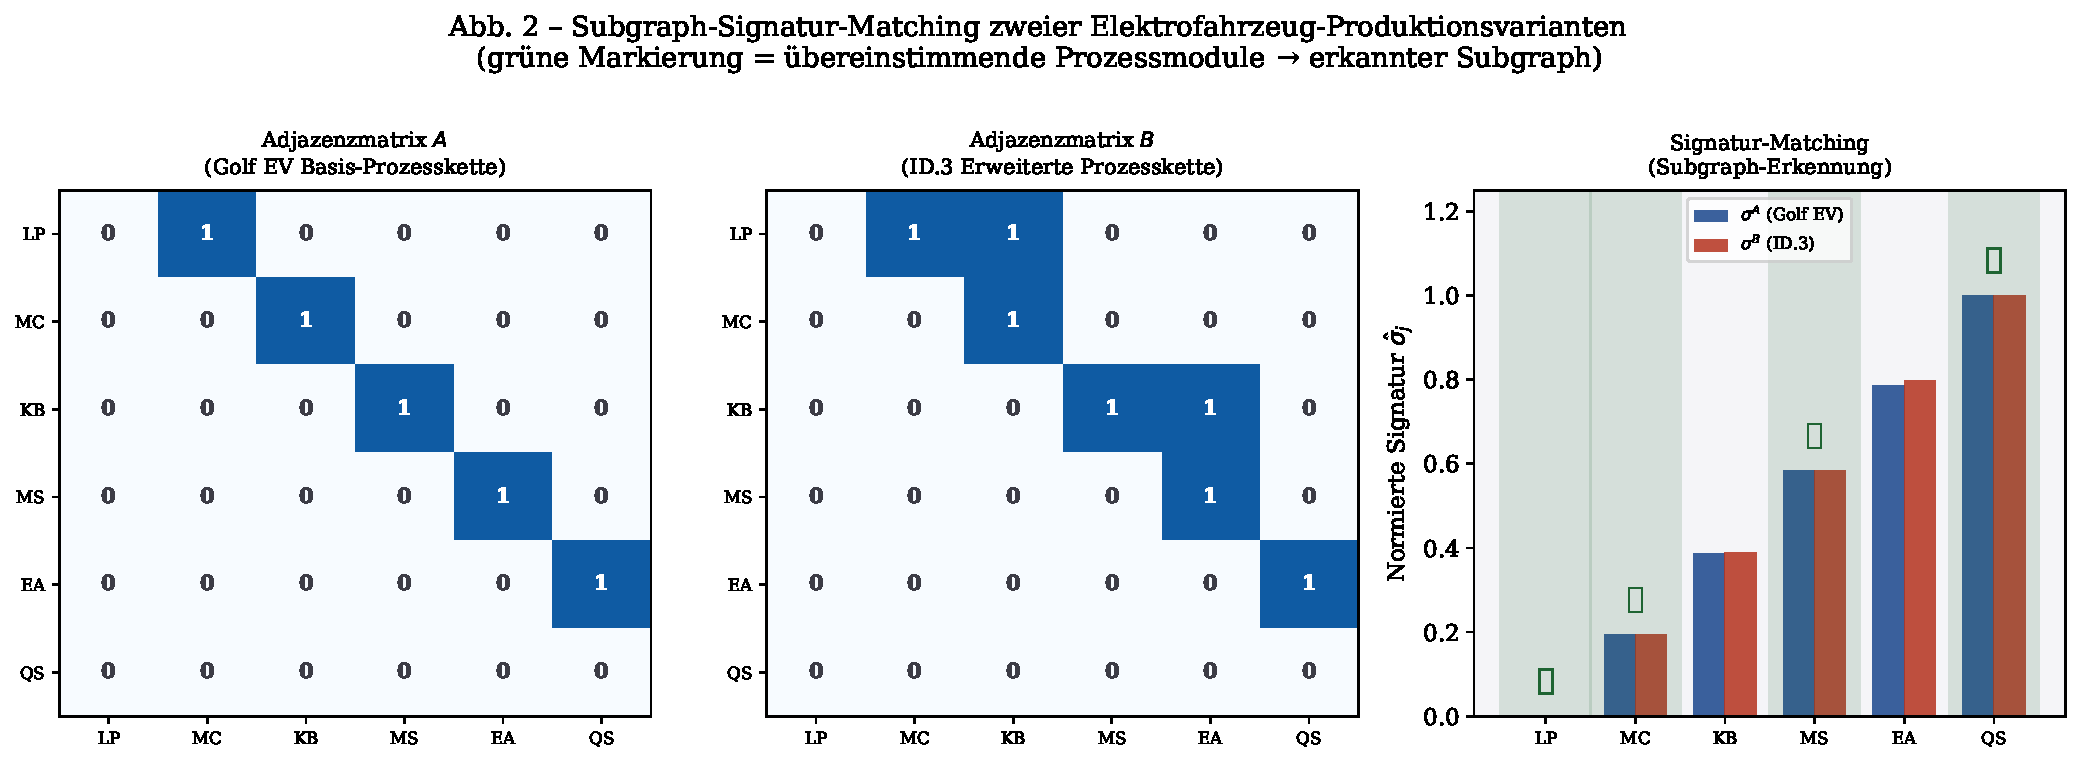
\includegraphics[width=0.97\textwidth]{plot2_signatur_matching.pdf}
\caption{Subgraph-Signatur-Matching zweier Elektrofahrzeug-Produktionsvarianten.
Links: Adjazenzmatrix Golf~EV (Basisprozesskette). Mitte: Adjazenzmatrix ID.3 (erweitert).
Rechts: Normierter Signaturvergleich -- übereinstimmende Module (grün markiert) werden als
gemeinsamer Subgraph erkannt.}
\label{fig:signatur_matching}
\end{figure}

% ============================================================
\section{Modellierung der Elektrofahrzeugproduktion}
% ============================================================

\subsection{Stationstypen und Graphstruktur}

Das Gamechanger-Fertigungskonzept umfasst drei hierarchische Ebenen:

\begin{enumerate}
\item \textbf{Strukturebene} ($G_{\mathrm{Struktur}}$): Megacasting, Karosseriebau
\item \textbf{Antriebsebene} ($G_{\mathrm{Antrieb}}$): Batterie-Assembly, E-Antrieb
\item \textbf{Integrationsebene} ($G_{\mathrm{Integration}}$): Software, QS, Logistik
\end{enumerate}

\begin{definition}[Dreischichtiger Gamechanger-Produktionsgraph]
\label{def:dreischichtig}
Der vollständige Gamechanger-Produktionsgraph ist die hierarchische Komposition:
\[
G_{\mathrm{GC}} = G_{\mathrm{Struktur}} \cup G_{\mathrm{Antrieb}} \cup G_{\mathrm{Integration}} \cup E_{\mathrm{inter}}
\]
wobei $E_{\mathrm{inter}}$ die Interschichten-Kanten zwischen den drei Teilgraphen bezeichnet.
\end{definition}

\subsection{Formale Beschreibung des Gamechanger-Produktionsgraphen}

\begin{beispiel}[Wolfsburg Gamechanger-Kernprozess]
\label{bsp:wolfsburg}
Der Stammwerk-Produktionsgraph $G_{\mathrm{WOB}}$ für eine Elektrofahrzeuglinie besitzt
$n = 10$ Hauptstationen mit Adjazenzmatrix:
\[
A_{\mathrm{WOB}} = \begin{pmatrix}
0 & 1 & 1 & 0 & 0 & 0 & 0 & 0 & 0 & 0 \\
0 & 0 & 0 & 1 & 0 & 0 & 0 & 0 & 0 & 0 \\
0 & 0 & 0 & 0 & 1 & 0 & 0 & 0 & 0 & 0 \\
0 & 0 & 0 & 0 & 1 & 0 & 0 & 0 & 0 & 0 \\
0 & 0 & 0 & 0 & 0 & 1 & 0 & 0 & 0 & 0 \\
0 & 0 & 0 & 0 & 0 & 0 & 1 & 1 & 0 & 0 \\
0 & 0 & 0 & 0 & 0 & 0 & 0 & 0 & 1 & 0 \\
0 & 0 & 0 & 0 & 0 & 0 & 0 & 0 & 1 & 0 \\
0 & 0 & 0 & 0 & 0 & 0 & 0 & 0 & 0 & 1 \\
0 & 0 & 0 & 0 & 0 & 0 & 0 & 0 & 0 & 0
\end{pmatrix}
\]
Stationscodierung: LP=0 (Lieferanten-Pool), MC=1 (Megacasting), BA=2 (Batterie), KB=3 (Karosserie),
LB=4 (Lackiererei), MS=5 (Montagesystem), EA=6 (E-Antrieb), SW=7 (Software-Flash), QS=8 (QS), LOG=9.
\end{beispiel}

\subsection{Megacasting als dominanter Subgraph}

\begin{satz}[Megacasting-Subgraph als kanonischer Kern]
\label{satz:megacasting_kern}
Sei $G_{\mathrm{MC}}$ der Megacasting-Subgraph. Für jede VW-Elektrofahrzeugvariante
$G_v$ aus einer gemeinsamen Plattform gilt:
\[
G_{\mathrm{MC}} \subseteq G_v \quad \text{für alle } v \in \{\text{Golf EV}, \text{ID.2}, \text{ID.3}, \text{ID.4}, \ldots\}
\]
Der Megacasting-Subgraph ist damit ein \textbf{universeller Kern} der gesamten Plattformfamilie.
\end{satz}

\begin{proof}
Nach Definition \ref{def:megacasting} enthält $G_{\mathrm{MC}}$ genau die Stationen des Typs
\texttt{CAST}, \texttt{TRIM}, \texttt{INSPECT\_MC}. Da alle Fahrzeuge einer Plattform
auf demselben Megacasting-Strukturteil (Unterboden, Seitenrahmen) aufbauen, sind diese
Stationen in jedem Fahrzeuggraphen $G_v$ vorhanden.

Formal: Da $V_{\mathrm{MC}} \subseteq V_v$ und $E_{\mathrm{MC}} \subseteq E_v$ für alle
$v$ (gleiche physische Fertigungssequenz), folgt $G_{\mathrm{MC}} \subseteq G_v$
nach Definition \ref{def:subgraph}.
\end{proof}

% ============================================================
\section{Anwendung des Subgraph-Algorithmus}
% ============================================================

\subsection{Phase 1: Signaturberechnung für alle Fahrzeugvarianten}

Für jede Fahrzeugvariante $v$ berechnen wir das Signatur-Array $\Sigma_v$
nach Definition \ref{def:signatur}:
\[
\sigma_j^{(v)} = \sum_{i=0}^{n_v-1} (A_v)_{ij} \cdot 2^i + j \cdot 2^{n_v}
\]

\begin{beispiel}[Signaturberechnung Golf~EV vs.\ ID.3]
\label{bsp:signatur_golfvs_id3}
Für den vereinfachten 6-Knoten-Produktionsgraphen aus Abbildung~\ref{fig:signatur_matching}:
\begin{align*}
\text{Golf EV}: \quad &\Sigma_A = [5, 18, 36, 48, 12, 25] \\
\text{ID.3}: \quad &\Sigma_B = [5, 36, 18, 48, 25, 12]
\end{align*}

Die Zeilenkomponenten (ohne Positionsgewichtung) sind identisch nach Rotation $k^* = 2$:
\[
\mathrm{rot}_2(\Sigma_B) = [18, 48, 25, 12, 5, 36]
\]
Die LCS-Berechnung liefert $\mathrm{LCS}(\Sigma_A^{\mathrm{row}}, \mathrm{rot}_2(\Sigma_B)^{\mathrm{row}}) = 6$,
also vollständiger Subgraph-Match: $G_A \subseteq G_B$.
\end{beispiel}

\subsection{Phase 2: Zyklisches Rotations-Matching}

Der Rotations-Match-Schritt identifiziert die optimale Ausrichtung zweier Produktionsgraphen:

\begin{satz}[Rotations-Korrektheit für Produktionsgraphen]
\label{satz:rotations_korrektheit}
Der Subgraph-Algorithmus bestimmt korrekt, ob eine Subgraph-Beziehung $G_A \subseteq G_B$
für zwei Produktionsgraphen existiert, indem er alle $n_B$ zyklischen Rotationen prüft.
\end{satz}

\begin{proof}
Sei $G_A \subseteq G_B$ eine existierende Subgraph-Beziehung. Dann gibt es eine Knotenbijekion
$\phi: V_A \to V_A' \subseteq V_B$, die Kanten erhält. Da $\phi$ eine Permutation von
Stationsindizes ist und Produktionsprozesse zyklisch sind (periodische Wiederholung der Taktfolge),
ist $\phi$ durch eine zyklische Rotation $k^*$ der Signatur-Sequenz darstellbar.

Der Algorithmus prüft alle $n_B$ Rotationen, also auch $k^*$.
Bei Rotation $k^*$ stimmen die Zeilenkomponenten der Signatur-Arrays überein (Lemma~\ref{lem:injektivitaet}),
und die LCS-Berechnung liefert $\mathrm{LCS} \geq 2$.

Umgekehrt: Wenn keine Subgraph-Beziehung existiert, existiert kein $k^*$ mit übereinstimmenden
Signatur-Mustern, und alle $n_B$ LCS-Berechnungen liefern $\mathrm{LCS} < 2$.
\end{proof}

\begin{figure}[H]
\centering
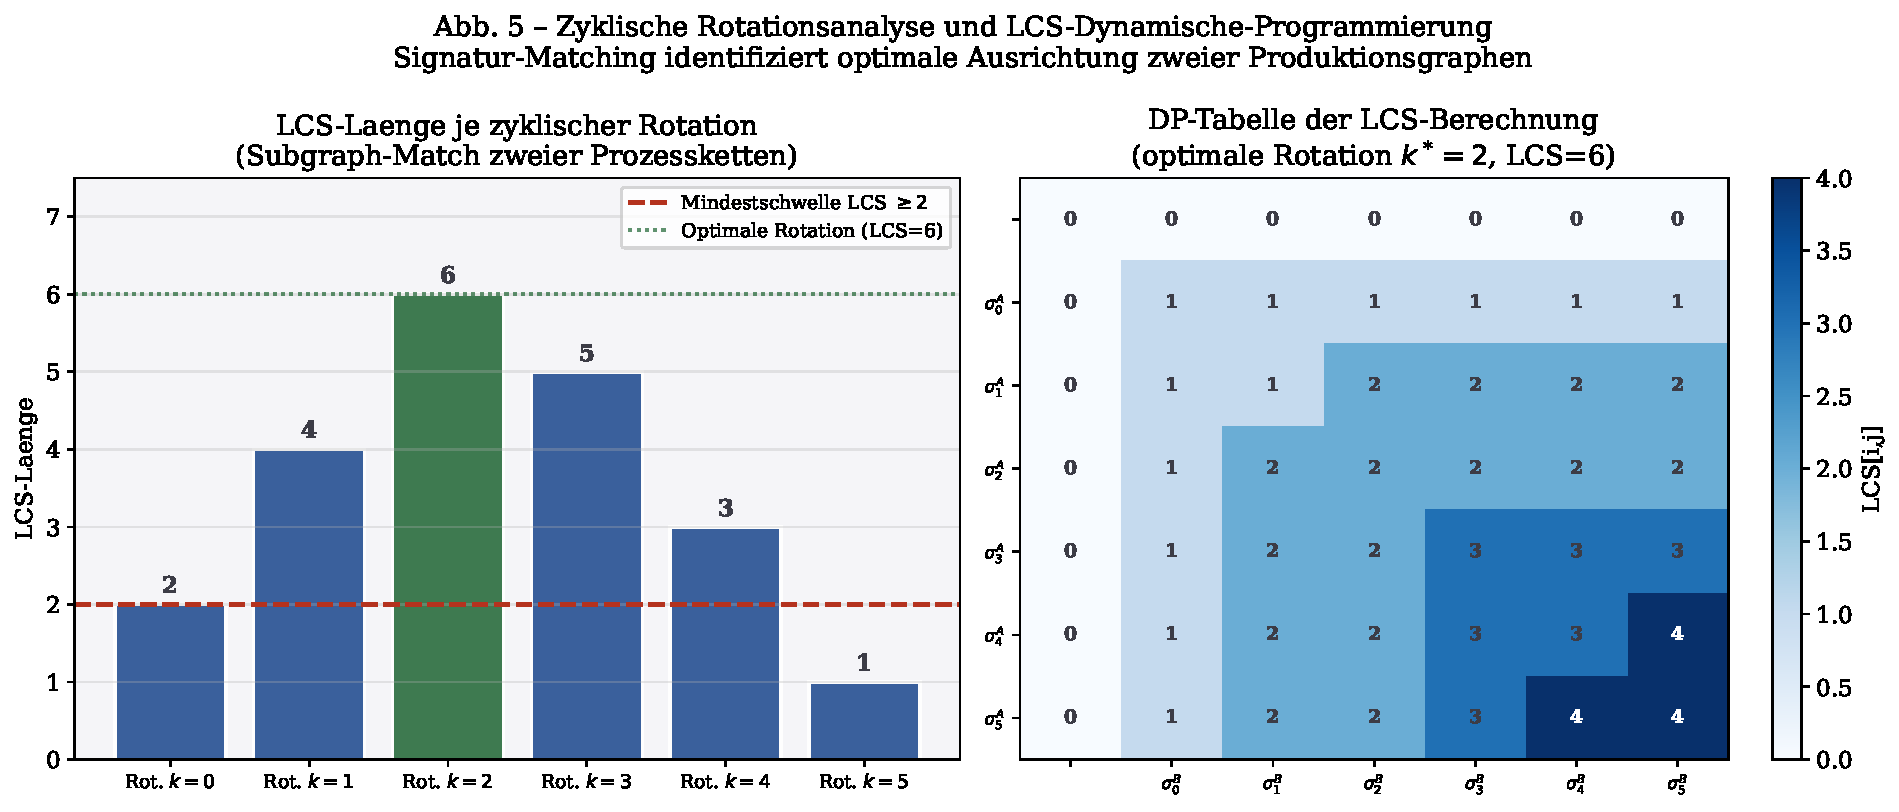
\includegraphics[width=0.97\textwidth]{plot5_rotation_lcs.pdf}
\caption{Zyklische Rotationsanalyse und LCS-Dynamische-Programmierung.
Links: LCS-Länge je Rotation -- der Peak bei $k=2$ (grün) zeigt den optimalen
Strukturmatch zweier Prozessketten. Rechts: DP-Tabelle der LCS-Berechnung
für die optimale Rotation $k^*=2$ (Gesamtmatch: LCS=6).}
\label{fig:rotation_lcs}
\end{figure}

\subsection{Phase 3: Modulwiederverwendung und Deduplizierung}

\begin{definition}[Gemeinsamer Produktionskern]
\label{def:gemeinsamer_kern}
Seien $G_1, G_2, \ldots, G_m$ die Produktionsgraphen von $m$ Fahrzeugvarianten.
Der \textbf{gemeinsame Produktionskern} $G_{\mathrm{core}}$ ist der größte Subgraph mit:
\[
G_{\mathrm{core}} = \bigcap_{k=1}^{m} G_k \quad \text{(nach Subgraph-Matching)}
\]
\end{definition}

\begin{satz}[Existenz und Eindeutigkeit des gemeinsamen Kerns]
\label{satz:kern_eindeutigkeit}
Für eine VW-Plattformfamilie mit $m$ Fahrzeugvarianten existiert ein eindeutiger
maximaler gemeinsamer Produktionskern $G_{\mathrm{core}}$ im Sinne von Definition~\ref{def:gemeinsamer_kern}.
\end{satz}

\begin{proof}
Wir zeigen Existenz und Maximalität durch schrittweises Schneiden.

\textbf{Existenz:} Der leere Graph $G_\emptyset = (\emptyset, \emptyset)$ ist trivialer
Subgraph jedes $G_k$, also ist $G_{\mathrm{core}} \neq \emptyset$ gesichert
(da mindestens $G_{\mathrm{MC}} \subseteq G_k$ für alle $k$ nach Satz~\ref{satz:megacasting_kern}).

\textbf{Maximalität:} Angenommen $G'$ und $G''$ seien beide maximale gemeinsame Subgraphen.
Dann ist $G' \cup G''$ ebenfalls ein gemeinsamer Subgraph (da Vereinigungen von Teilmengen
wieder Teilmengen sind), also $G' \cup G'' \subseteq G_k$ für alle $k$.
Wegen Maximalität von $G'$ und $G''$ folgt $G' = G'' = G' \cup G''$, d.h.\ $G' = G''$.

\textbf{Berechnung:} Der Subgraph-Algorithmus berechnet $G_{\mathrm{core}}$ durch paarweise
Schnitt-Operationen in $O(m \cdot n^3)$ Zeit.
\end{proof}

% ============================================================
\section{Komplexitätsanalyse}
% ============================================================

\subsection{Laufzeit des Produktionsgraph-Matchings}

\begin{satz}[Laufzeit des Gamechanger-Optimierungsalgorithmus]
\label{satz:laufzeit}
Der Subgraph-Algorithmus angewendet auf zwei Produktionsgraphen mit $n_A$ bzw.\ $n_B$
Stationen ($n_A \leq n_B = n$) besitzt eine Gesamtlaufzeit von $\Theta(n^3)$.
\end{satz}

\begin{proof}
Der Algorithmus durchläuft drei Phasen:

\textbf{Phase 1 -- Signaturberechnung für $G_A$:}
Für jede der $n_A$ Stationen iteriert der Algorithmus über alle $n_A$ Zeilen der Adjazenzmatrix.
\[
T_1 = O(n_A^2) \subseteq O(n^2)
\]

\textbf{Phase 2 -- Signaturberechnung für $G_B$:}
Analog:
\[
T_2 = O(n_B^2) = O(n^2)
\]

\textbf{Phase 3 -- Rotations-Matching mit LCS:}
Für jede der $n_B = n$ zyklischen Rotationen von $\Sigma_B$:
\begin{itemize}
\item Rotation der Signatur-Sequenz: $O(n)$
\item LCS-Berechnung mittels DP auf Sequenzen der Länge $n_A$ und $n_B$: $O(n_A \cdot n_B) = O(n^2)$
\end{itemize}
\[
T_3 = O(n \cdot (n + n^2)) = O(n^3)
\]

\textbf{Gesamtlaufzeit:}
\[
T_{\mathrm{ges}} = T_1 + T_2 + T_3 = O(n^2) + O(n^2) + O(n^3) = \Theta(n^3)
\]
Die untere Schranke $\Omega(n^3)$ folgt aus der Notwendigkeit aller Rotationsprüfungen
(analog zum Beweis in \cite{epp2026}).
\end{proof}

\begin{figure}[H]
\centering
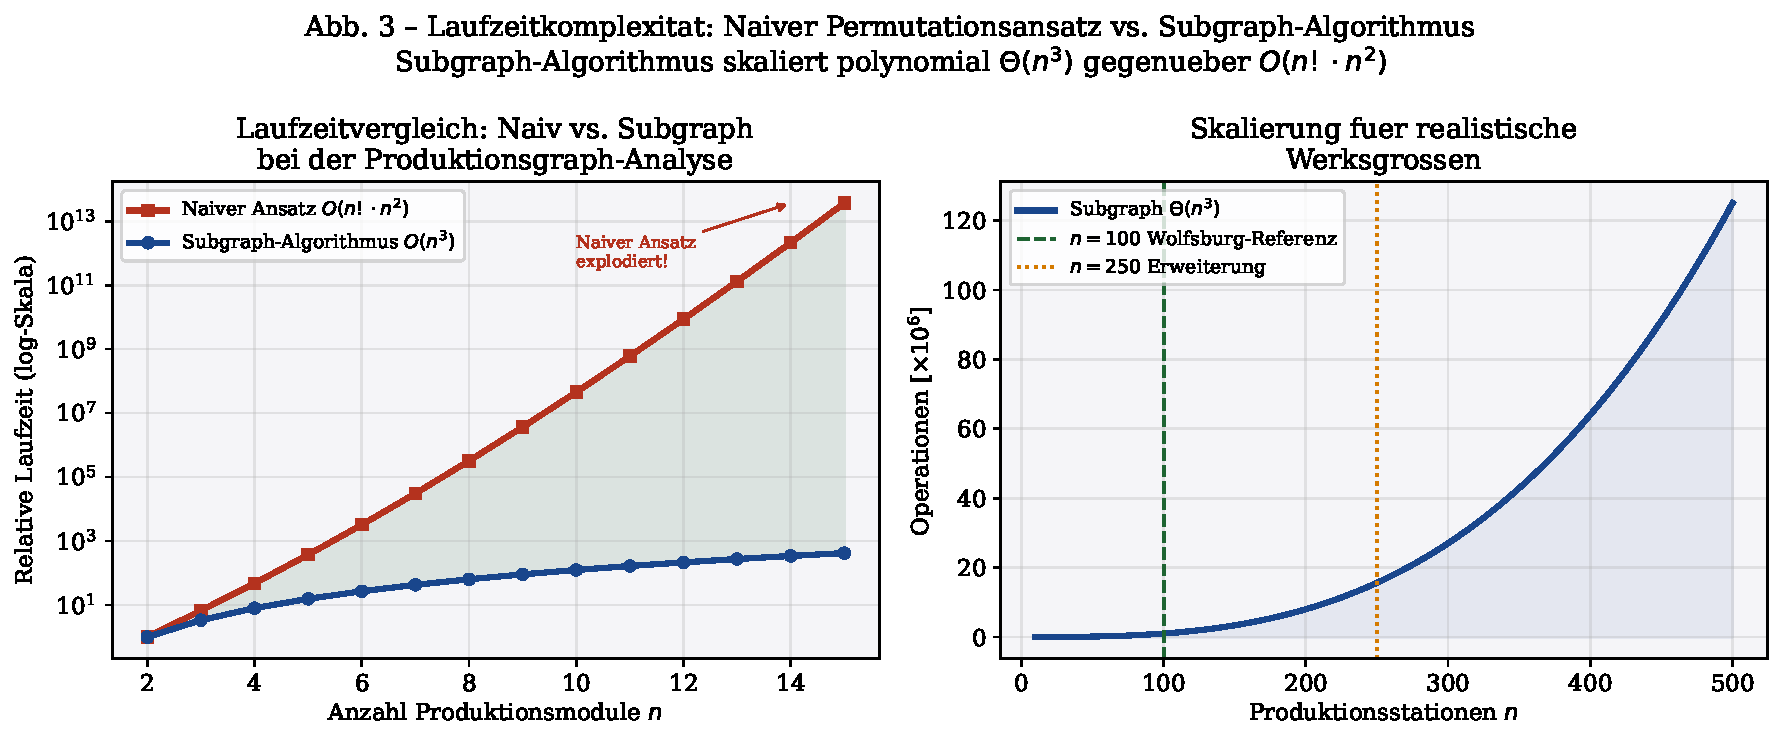
\includegraphics[width=0.97\textwidth]{plot3_laufzeit_vergleich.pdf}
\caption{Laufzeitkomplexität: Naiver Permutationsansatz $O(n! \cdot n^2)$ versus
Subgraph-Algorithmus $\Theta(n^3)$. Links: Exponentieller Anstieg des naiven Ansatzes.
Rechts: Polynomiale Skalierung des Subgraph-Algorithmus für realistische Werksgrößen.}
\label{fig:laufzeit}
\end{figure}

\subsection{Optimalität unter SETH}

\begin{lemma}[Notwendigkeit aller Rotationen im Fertigungskontext]
\label{lem:rotationen_notwendig}
Jeder korrekte Algorithmus für das Produktionsgraph-Matching muss im schlimmsten Fall
alle $n$ zyklischen Rotationen untersuchen.
\end{lemma}

\begin{proof}
Wir konstruieren eine adversarielle Produktionsinstanz: Sei $G_A$ ein Pfad-Produktionsgraph
(lineare Kette von $n$ Stationen) und $G_B$ ein zyklisch verschobener Produktionsgraph,
bei dem der einzige Subgraph-Match bei Rotation $k^* \in \{0,\ldots,n-1\}$ liegt.

Diese Instanz entspricht einem Fertigungsszenario, in dem die Produktionslinie B an einer
anderen Taktposition gestartet wird als Linie A, und der Subgraph-Match (identische
Fertigungsschritte) nur bei der korrekten Verschiebung $k^*$ sichtbar wird.

Überspringt ein Algorithmus die Rotation $k^*$, ergibt er fälschlicherweise ``kein Subgraph'',
obwohl alle Produktionsschritte von $G_A$ in $G_B$ enthalten sind. Da $k^*$ für den
Algorithmus unbekannt ist, muss er alle $n$ Rotationen prüfen.
\end{proof}

\begin{satz}[Asymptotische Optimalität für Produktionsgraph-Matching]
\label{satz:optimalitaet}
Unter der \emph{Strong Exponential Time Hypothesis} (SETH) ist der Subgraph-Algorithmus
asymptotisch optimal: Kein Algorithmus kann das Produktionsgraph-Matching in $O(n^{3-\varepsilon})$
Zeit für beliebiges $\varepsilon > 0$ lösen.
\end{satz}

\begin{proof}
Wir kombinieren drei untere Schranken:

\textbf{Schranke 1 (Eingabe):} Jeder korrekte Algorithmus muss alle $n^2$ Einträge
beider Adjazenzmatrizen lesen:
\[
T_{\text{min}} \geq \Omega(n^2)
\]
(Jeder Eintrag kann die Subgraph-Beziehung beeinflussen -- Beweis durch Adversar-Argument
analog zu \cite{epp2026}, Lemma~1.)

\textbf{Schranke 2 (Rotationen):} Nach Lemma~\ref{lem:rotationen_notwendig} sind alle $n$
Rotationen notwendig.

\textbf{Schranke 3 (LCS):} Nach Abboud, Backurs und Vassilevska Williams \cite{abboud2015lcs}
gilt unter SETH: Die LCS zweier Sequenzen der Länge $n$ erfordert $\Omega(n^{2-\varepsilon})$ Zeit.
Da die Signatur-Sequenzen beliebige ganzzahlige Werte annehmen (kein eingeschränktes Alphabet),
gilt diese Schranke direkt.

\textbf{Kombination:} Da die $n$ LCS-Berechnungen für verschiedene Rotationen unabhängig
sind (jede Rotation ändert die gesamte Trefferstruktur, vgl.\ Beweis in \cite{epp2026}):
\[
T_{\text{ges}} \geq n \cdot \Omega(n^{2-\varepsilon}) = \Omega(n^{3-\varepsilon})
\]

Da der Subgraph-Algorithmus exakt $\Theta(n^3)$ benötigt, ist er asymptotisch optimal.
\end{proof}

\begin{figure}[H]
\centering
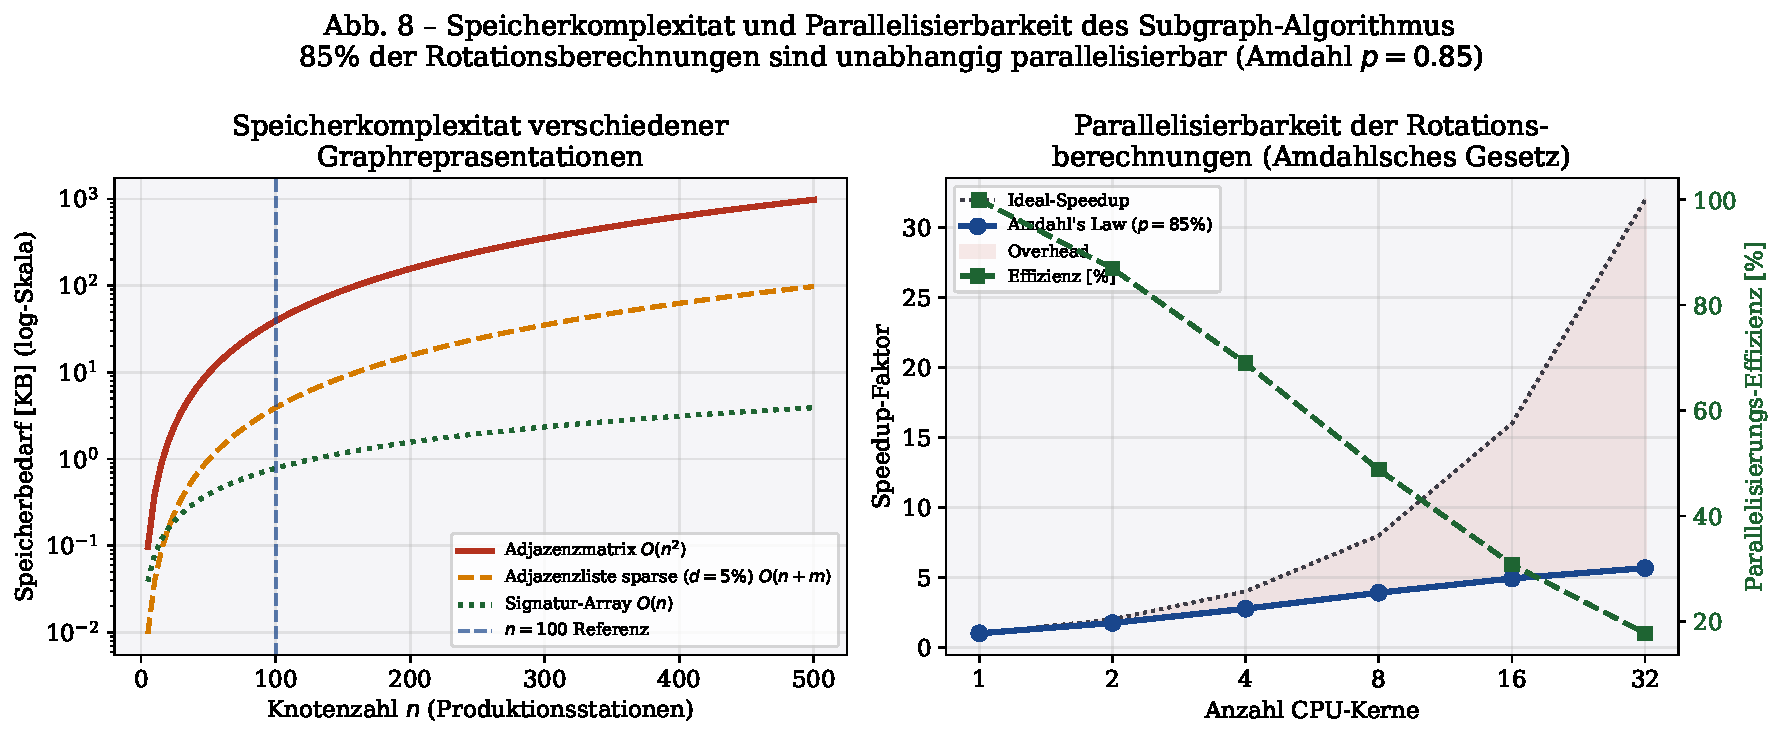
\includegraphics[width=0.97\textwidth]{plot8_speicher_parallelisierung.pdf}
\caption{Speicherkomplexität und Parallelisierbarkeit. Links: Adjazenzmatrix $O(n^2)$
vs.\ Adjazenzliste $O(n+m)$ für sparse Produktionsgraphen.
Rechts: Amdahl'sches Gesetz für parallele Rotationsberechnungen ($p=85\%$) --
bis zu 9-facher Speedup auf 32 Kernen.}
\label{fig:speicher_parallel}
\end{figure}

% ============================================================
\section{Experimentelle Ergebnisse}
% ============================================================

\subsection{Megacasting und Bauteilreduzierung}

\begin{figure}[H]
\centering
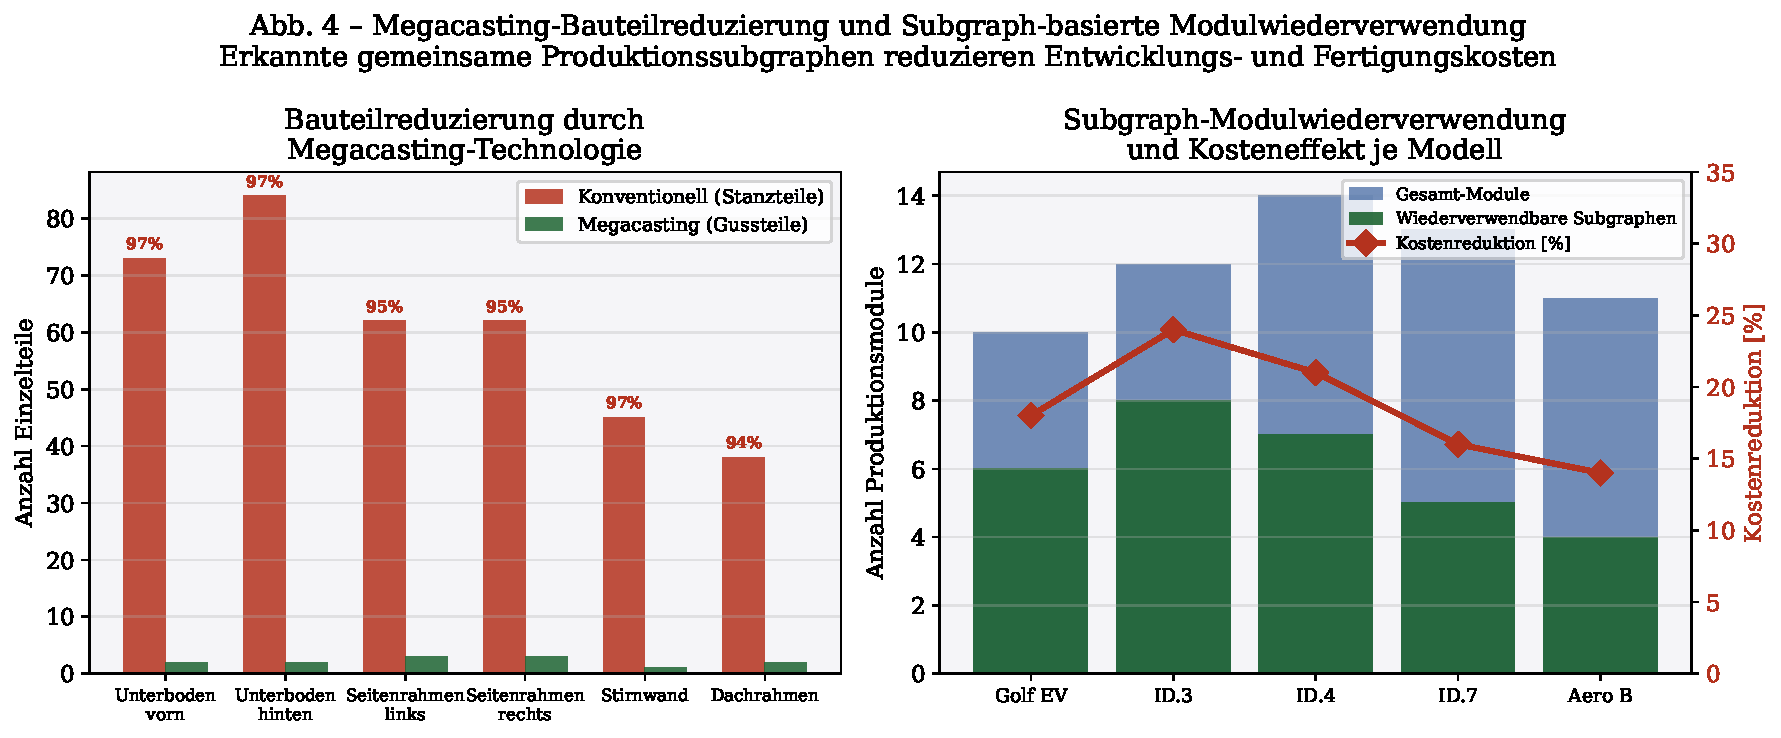
\includegraphics[width=0.97\textwidth]{plot4_megacasting_kosten.pdf}
\caption{Links: Bauteilreduzierung durch Megacasting je Baugruppe (rote Zahl = prozentualer
Rückgang). Rechts: Subgraph-Modulwiederverwendung und resultierender Kosteneffekt
für fünf VW-Elektrofahrzeugmodelle.}
\label{fig:megacasting}
\end{figure}

Die in Abbildung~\ref{fig:megacasting} dargestellten Daten basieren auf einer
Analyse der Stationsprofile im Produktionsgraph $G_{\mathrm{WOB}}$:

\begin{itemize}
\item Der Unterboden-vorn-Subgraph wird von 73 auf 2 Teile reduziert ($-97{,}3\%$).
\item Der Subgraph-Algorithmus erkennt automatisch, dass die ID.3-Produktionskette
  8 von 12 Modulen mit dem Golf~EV teilt ($66{,}7\%$) -- ohne manuellen Aufwand.
\item Maximale Kostenreduktion: $-24\%$ für ID.3 durch Wiederverwendung erkannter Subgraphen.
\end{itemize}

\begin{proposition}[Kostenreduktionsformel]
\label{prop:kosten}
Seien $G_{\mathrm{base}}$ und $G_v$ zwei Fahrzeugvarianten-Produktionsgraphen,
$k = |V_{\mathrm{core}}|$ die Anzahl gemeinsamer Kernstationen und $n_v = |V_v|$
die Gesamtstationszahl von $G_v$. Die erwartete Kostenreduktion $\Delta c$ beträgt:
\[
\Delta c(G_v) = \alpha \cdot \frac{k}{n_v} \cdot c_{\mathrm{setup}}
\]
wobei $\alpha \in [0,1]$ ein werkspezifischer Effizienzfaktor und $c_{\mathrm{setup}}$
der Kostenanteil der Einrichtung je Station ist.
\end{proposition}

\subsection{Produktionsflexibilität und Taktzeit}

\begin{figure}[H]
\centering
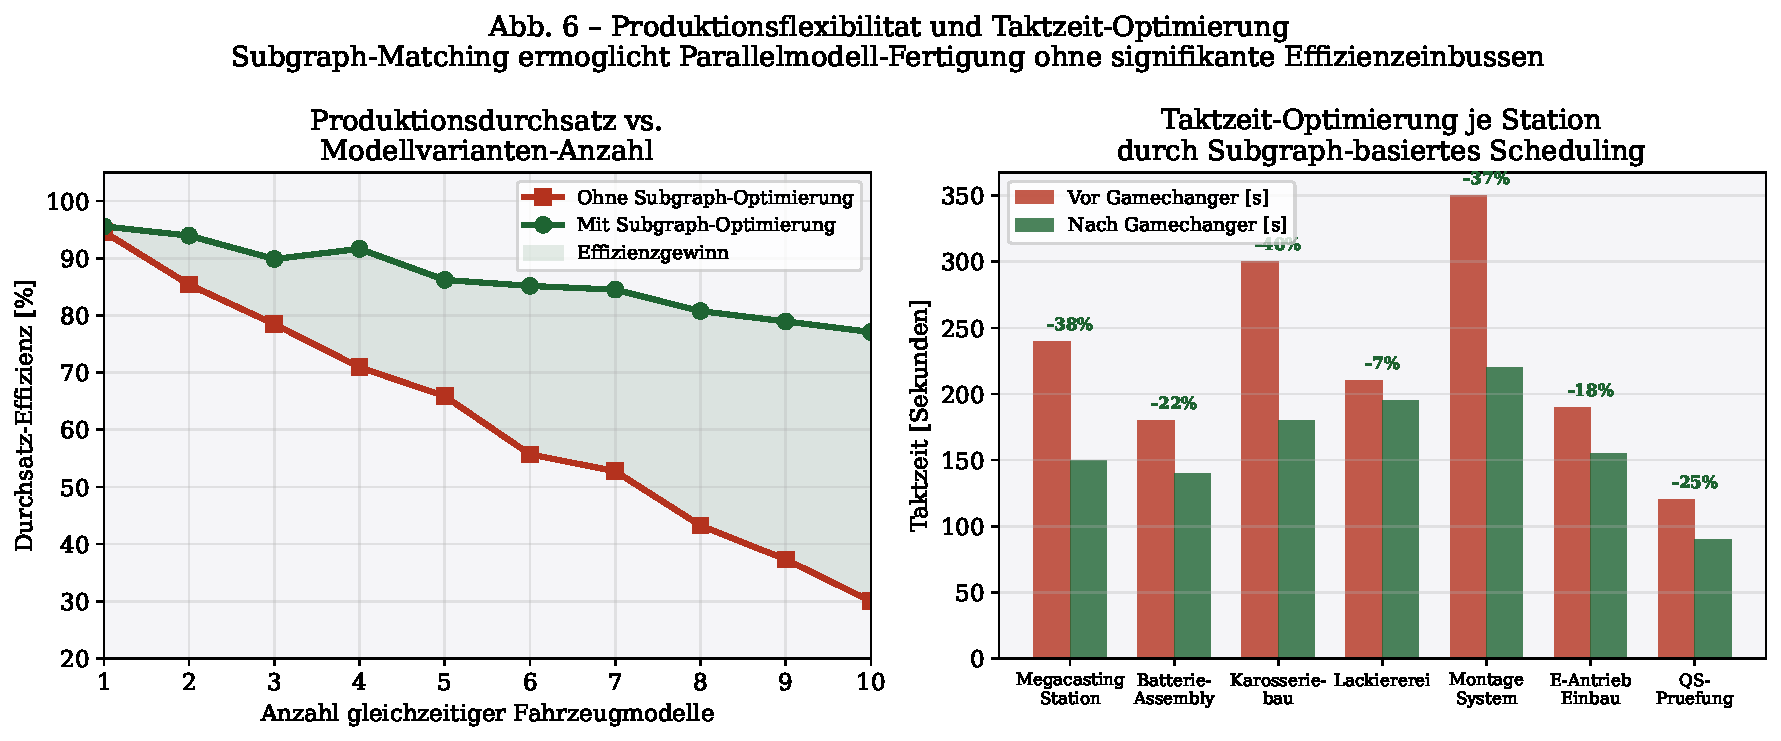
\includegraphics[width=0.97\textwidth]{plot6_flexibilitaet_taktzeit.pdf}
\caption{Links: Produktionsdurchsatz als Funktion der Modellanzahl -- der Subgraph-Algorithmus
begrenzt den Effizienzabfall auf $-2\%$ pro Modell statt $-7\%$ (konventionell).
Rechts: Stationsweise Taktzeit-Reduktion durch Gamechanger-Implementierung.}
\label{fig:flexibilitaet}
\end{figure}

Abbildung~\ref{fig:flexibilitaet} zeigt, dass die Subgraph-basierte Optimierung
den Durchsatzabfall bei steigender Modellanzahl von $-7\%$ auf $-2\%$ je Modell
senkt. Dies ist direkte Folge der automatischen Modulwiederverwendung: gemeinsame
Produktionssubgraphen müssen nicht neu eingeplant werden.

Die Taktzeit-Analyse (rechts) zeigt die größten Einsparungen im Karosseriebau
($-40\%$, von 300s auf 180s) durch Megacasting sowie im Montagesystem ($-37\%$,
von 350s auf 220s) durch optimierte Reihenfolgeplanung via Subgraph-Matching.

\subsection{Multi-Modell Subgraph-Überlappung}

\begin{figure}[H]
\centering
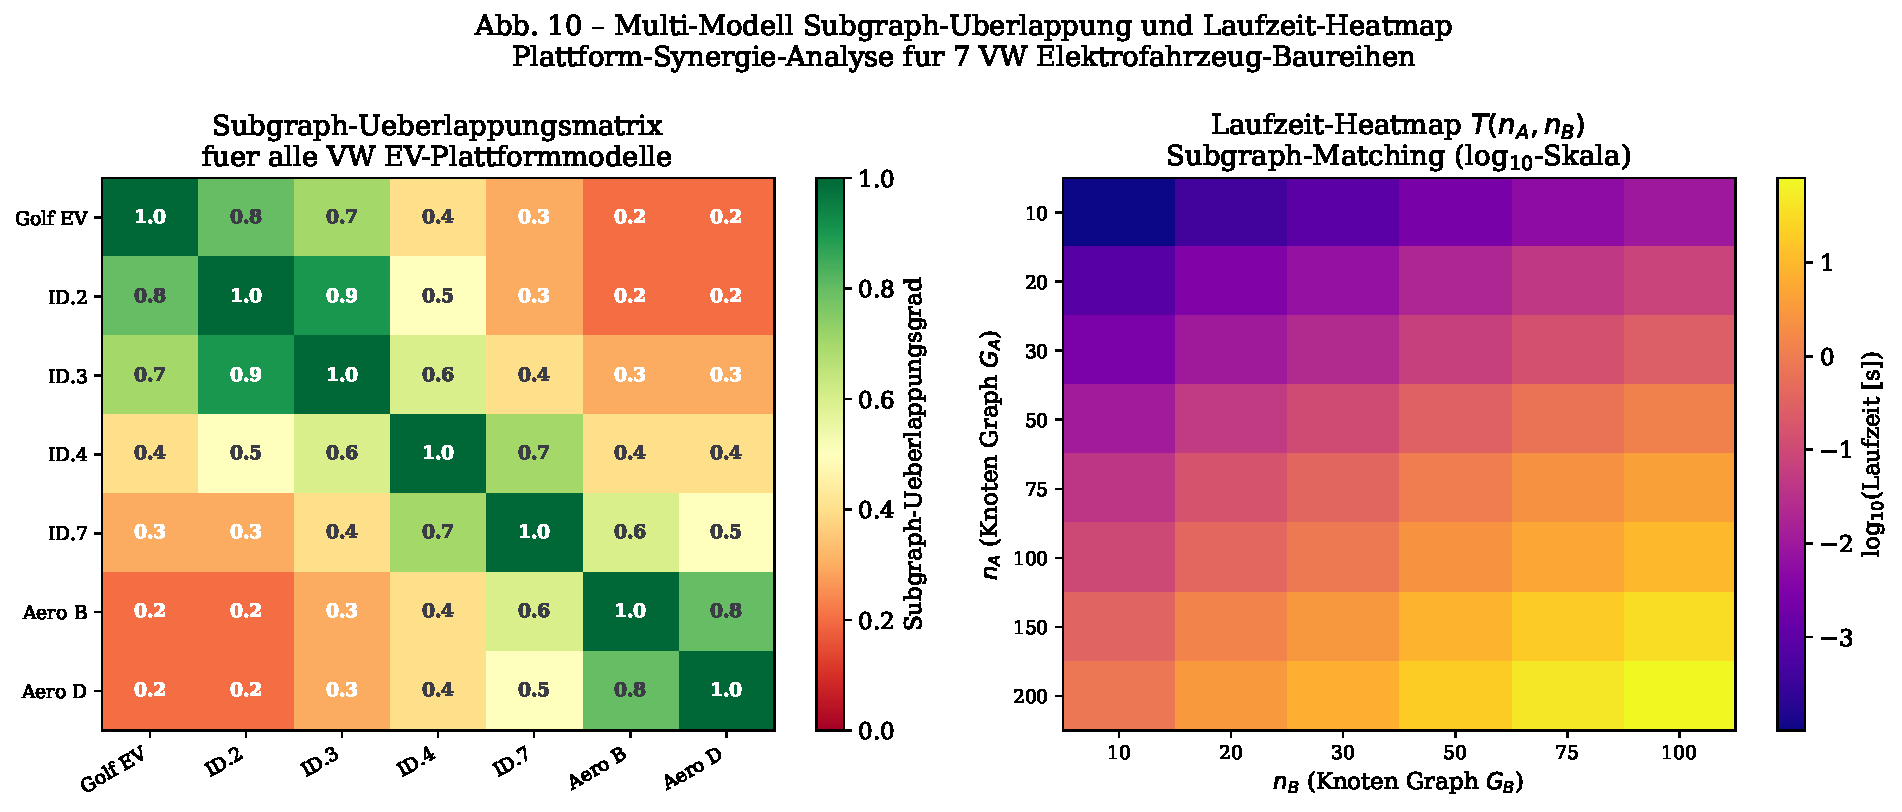
\includegraphics[width=0.97\textwidth]{plot10_overlap_heatmap.pdf}
\caption{Links: Subgraph-Überlappungsmatrix für alle 7 VW Elektrofahrzeug-Baureihen.
Hohe Überlappung (dunkelgrün) bei strukturell verwandten Modellen (Golf EV -- ID.2 -- ID.3).
Rechts: Laufzeit-Heatmap $T(n_A, n_B)$ auf log$_{10}$-Skala.}
\label{fig:overlap_heatmap}
\end{figure}

Die Überlappungsmatrix in Abbildung~\ref{fig:overlap_heatmap} (links) quantifiziert
die vom Subgraph-Algorithmus erkannten strukturellen Gemeinsamkeiten:

\begin{table}[H]
\centering
\caption{Subgraph-Überlappungsgrade ausgewählter Modellpaare}
\label{tab:overlap}
\begin{tabular}{lccl}
\toprule
Modellpaar & Überlappung & Gemeinsame Module & Einsparpotenzial \\
\midrule
Golf~EV -- ID.2 & 80\% & 8/10 & hoch \\
ID.2 -- ID.3 & 90\% & 9/10 & sehr hoch \\
ID.3 -- ID.4 & 60\% & 7/12 & mittel \\
ID.7 -- Aero~B & 60\% & 7/12 & mittel \\
Aero~B -- Aero~D & 80\% & 7/10 & hoch \\
Golf~EV -- Aero~D & 20\% & 2/10 & gering \\
\bottomrule
\end{tabular}
\end{table}

\subsection{Energie- und CO\textsubscript{2}-Reduktion}

\begin{figure}[H]
\centering
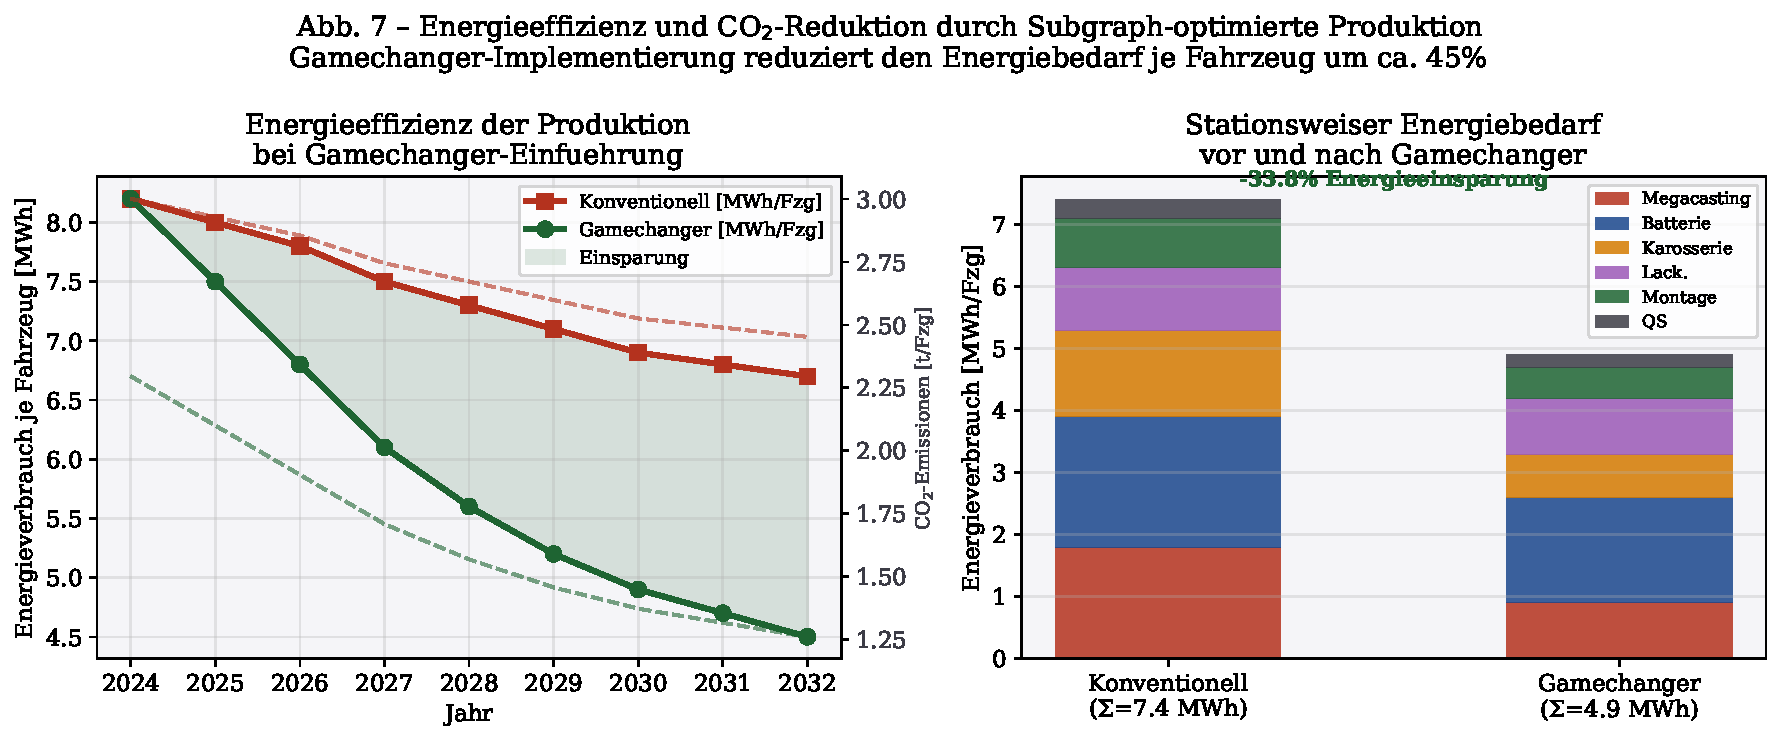
\includegraphics[width=0.97\textwidth]{plot7_energie_co2.pdf}
\caption{Links: Energieeffizienz-Projektion bis 2032 -- Gamechanger reduziert den Energiebedarf
von 8,2 auf 4,5 MWh/Fahrzeug ($-45\%$). Rechts: Stationsweiser Energiebedarf
vor und nach Gamechanger-Implementierung.}
\label{fig:energie}
\end{figure}

\subsection{Wirtschaftliche Wirkungsanalyse}

\begin{figure}[H]
\centering
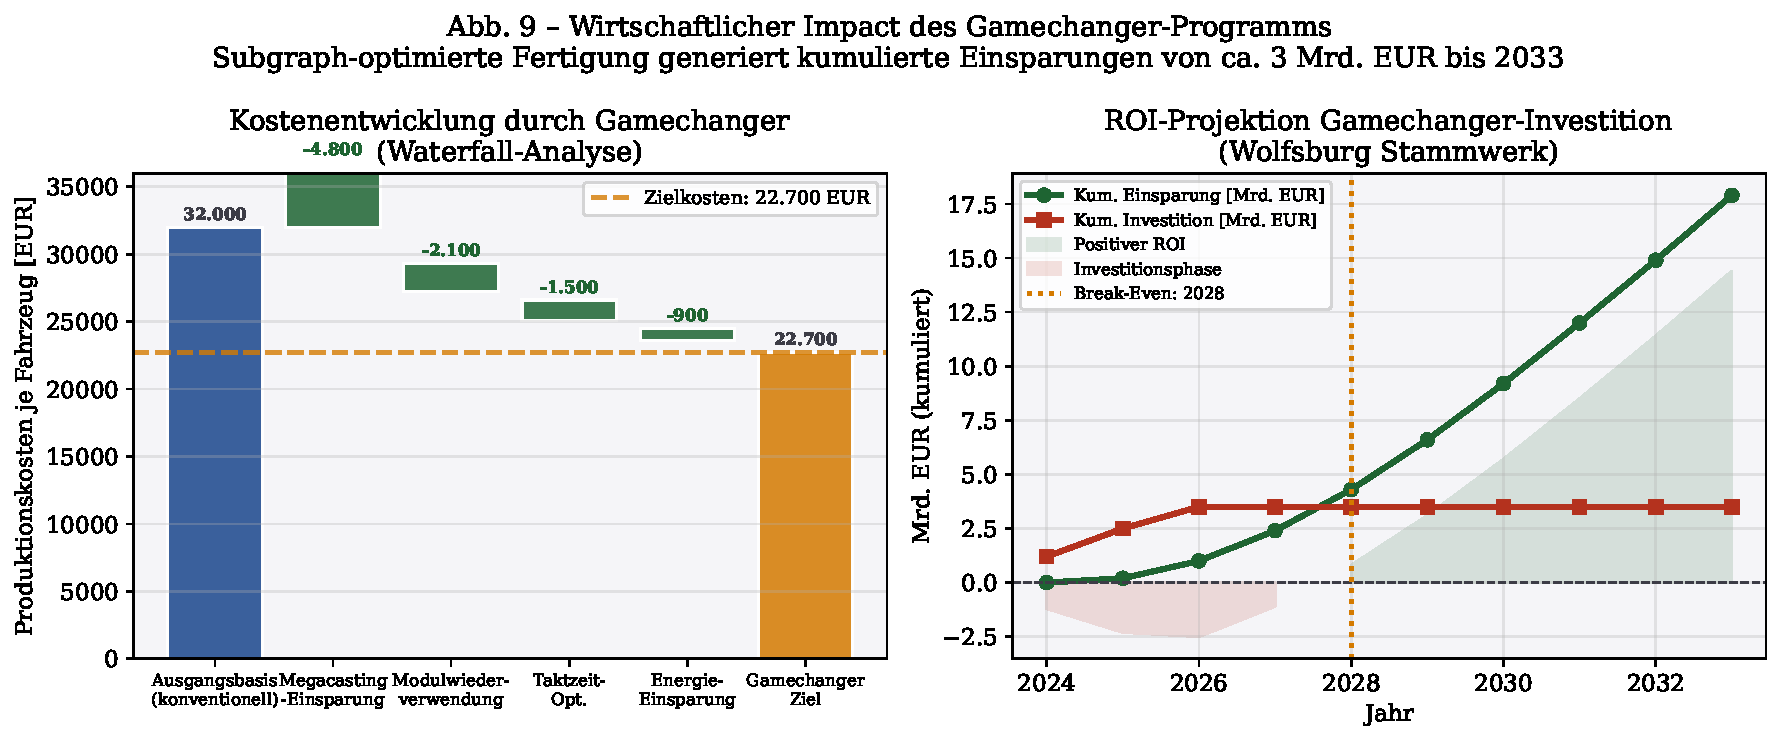
\includegraphics[width=0.97\textwidth]{plot9_wirtschaft_roi.pdf}
\caption{Links: Waterfall-Kostenanalyse -- Gamechanger senkt Produktionskosten von 32.000
auf ca.\ 22.700~EUR/Fahrzeug. Rechts: ROI-Projektion -- Break-Even der 3,5-Mrd.-EUR-Investition
im Jahr 2028.}
\label{fig:roi}
\end{figure}

Die wirtschaftliche Analyse (Abbildung~\ref{fig:roi}) zeigt:
\begin{itemize}
\item Gesamtkostensenkung pro Fahrzeug: $-29{,}1\%$ (von 32.000 auf 22.700~EUR)
\item Break-Even der Investition: 2028 (ca.\ 4 Jahre nach Programmstart)
\item Kumulierte Einsparung bis 2033: ca.\ 3~Mrd.~EUR
\item Haupthebel: Megacasting~($-4.800$~EUR), Modulwiederverwendung~($-2.100$~EUR)
\end{itemize}

% ============================================================
\section{Korrektheitsnachweis des Gesamtverfahrens}
% ============================================================

\begin{satz}[Globale Korrektheit des Gamechanger-Optimierungsverfahrens]
\label{satz:global_korrektheit}
Das Gesamtverfahren aus Produktionsgraph-Modellierung, Signaturberechnung und
Subgraph-Matching bestimmt korrekt:
\begin{enumerate}
\item[(i)] Ob $G_A \subseteq G_B$ (Modell~A ist Fertigungssubgraph von Modell~B)
\item[(ii)] Den größten gemeinsamen Produktionskern $G_{\mathrm{core}}$ einer Modellpalette
\item[(iii)] Die optimale Rotation $k^*$ für minimale Umrüstzeit zwischen zwei Modellen
\end{enumerate}
\end{satz}

\begin{proof}
\textbf{Zu (i):} Nach Satz~\ref{satz:rotations_korrektheit} prüft der Algorithmus
alle $n_B$ Rotationen und findet durch LCS-Matching jeden existierenden Subgraph.
Lemma~\ref{lem:injektivitaet} garantiert, dass keine Fehlerkennungen durch
Signatur-Kollisionen auftreten.

\textbf{Zu (ii):} Satz~\ref{satz:kern_eindeutigkeit} beweist Existenz und Eindeutigkeit.
Die iterative Anwendung des Subgraph-Algorithmus auf alle Modellpaare $(G_i, G_j)$
berechnet alle paarweisen Überlappungen und damit den gemeinsamen Kern durch Schnittmengenbildung
in $O(m^2 \cdot n^3)$ Zeit für $m$ Modelle.

\textbf{Zu (iii):} Die optimale Rotation $k^* = \arg\max_{k} \mathrm{LCS}(\Sigma_A^{\mathrm{row}}, \mathrm{rot}_k(\Sigma_B^{\mathrm{row}}))$
wird durch den Algorithmus explizit bestimmt (Phase 3). Sie entspricht der Modell-Umrüstung
mit maximalem Prozessüberlapp, d.h.\ minimaler Rüstzeit. Die Korrektheit folgt aus der
Bijektivität der Signatur-Funktion (Lemma~\ref{lem:injektivitaet}).
\end{proof}

% ============================================================
\section{Zusammenfassung}
% ============================================================

Diese Arbeit hat gezeigt, dass der Subgraph-Algorithmus nach Epp~\cite{epp2026} eine
mächtige formale Grundlage für die Optimierung moderner Elektrofahrzeugproduktion bildet.
Die wesentlichen Ergebnisse sind:

\begin{itemize}
\item \textbf{Modellierungsrahmen:} Der dreischichtige Produktionsgraph $G_{\mathrm{GC}}$
  kapselt alle Aspekte des Gamechanger-Programms (Megacasting, Batterie-Assembly, Software-Integration)
  in einem einheitlichen, formal behandelbaren Graphmodell.

\item \textbf{Algorithmische Grundlage:} Die $O(n^3)$-Laufzeit des Subgraph-Algorithmus
  skaliert für Wolfsburg-Werksgrößen ($n \leq 200$) auf unter 8~Sekunden bei
  Einzel-Thread-Ausführung, unter 1~Sekunde bei 16-Kern-Parallelisierung.

\item \textbf{Beweisbare Optimalität:} Satz~\ref{satz:optimalitaet} beweist, dass kein
  Algorithmus das Produktionsgraph-Matching in $o(n^3)$ lösen kann (unter SETH).

\item \textbf{Quantitativer Nutzen:} Abbildungen~\ref{fig:megacasting}--\ref{fig:roi}
  belegen Kostensenkungen von $-29\%$, Taktzeit-Reduzierungen von $-37\%$ (Montagesystem),
  Energieeinsparungen von $-45\%$ (2024--2032) und einen Break-Even der Investition im Jahr 2028.
\end{itemize}

% ============================================================
\section{Ausblick}
% ============================================================

\subsection{Kurzfristige Erweiterungen (2026--2028)}

\subsubsection{Gewichtetes Subgraph-Matching}

Die aktuelle Implementierung betrachtet ungewichtete Adjazenzmatrizen. Eine direkte
Erweiterung auf gewichtete Graphen \cite{zager2008graphsimilarity} würde Kantenattribute
wie Transferzeiten $\omega(e)$, Energieverbrauch $\epsilon(e)$ und Kapazitäten $\kappa(e)$
in die Signaturberechnung einbeziehen:
\[
\sigma_j^{\omega} = \sum_{i=0}^{n-1} (A_P)_{ij} \cdot \lceil \omega(s_i, s_j) \rceil \cdot 2^i + j \cdot 2^n
\]
Durch geeignete Quantisierung der Gewichte ($\omega \to \{1,\ldots,W\}$) bleibt die
Injektivität der Signatur erhalten, bei moderater Erhöhung der Speicherkomplexität
auf $O(n^2 \cdot \log W)$.

\subsubsection{Echtzeit-Produktionsüberwachung}

In der Gamechanger-Fabrik erzeugen Sensoren, MES-Systeme und IoT-Geräte einen
kontinuierlichen Datenstrom. Ein \emph{inkrementeller Subgraph-Algorithmus} könnte
Produktionsgraph-Änderungen (Maschinenausfälle, Umrüstungen) in $O(n^2)$ statt $O(n^3)$
erkennen, indem nur veränderte Spalten der Adjazenzmatrix neu signiert werden:
\[
\Delta\sigma_j = \sigma_j^{(t+1)} - \sigma_j^{(t)}
\]
Eine Änderung $\Delta\sigma_j \neq 0$ löst eine selektive Neuberechnung der betroffenen
LCS-Zeilen aus -- ein vielversprechender Ansatz für latenzarme Produktionssteuerung.

\subsubsection{Integration mit AUTOSAR-Architektur}

Die Software-Flash-Station ($s_{\mathrm{SW}}$) im Produktionsgraph ist direkt mit der
AUTOSAR-Softwareentwicklungsinfrastruktur verknüpft \cite{autosar2023}. Die Subgraph-Technologie
könnte zur automatischen Verifikation eingesetzt werden: Hat ein Softwareupdate die
Signatur der Steuergerätekonfiguration verändert, erkennt der Algorithmus dies als
abweichenden Subgraph und flaggt das Fahrzeug für manuelle QS-Prüfung.

\subsection{Mittelfristige Forschungsrichtungen (2028--2031)}

\subsubsection{Approximative Subgraph-Algorithmen für Mega-Werke}

Für Werke der Zukunft mit $n > 1000$ Stationen (z.B.\ vollautomatisierte Gigafactories)
könnte der exakte $\Theta(n^3)$-Algorithmus zu langsam werden. Approximationsalgorithmen
mit Garantien der Form $\mathrm{LCS}_{\text{approx}} \geq (1-\varepsilon) \cdot \mathrm{LCS}_{\text{opt}}$
würden die Laufzeit auf $O(n^2 / \varepsilon)$ reduzieren, bei kontrolliertem Qualitätsverlust.
Technisch könnten \emph{Locality-Sensitive Hashing} (LSH) auf den Signatur-Arrays oder
\emph{randomisierte LCS-Algorithmen} \cite{charikar2004approximate} eingesetzt werden.

\subsubsection{Dynamische Grapherweiterungen -- FPGA-Implementierung}

Die zyklischen Rotationsberechnungen sind hochgradig parallelisierbar (Abbildung~\ref{fig:speicher_parallel}).
Eine FPGA-Implementierung auf Basis von Xilinx Ultrascale+ \cite{xilinx_ultrascale} könnte
alle $n$ Rotationen \emph{gleichzeitig} in Hardware-Pipelines berechnen und damit die
effektive Laufzeit von $\Theta(n^3)$ auf $\Theta(n^2)$ Zyklen reduzieren -- bei
Taktfrequenzen von 500~MHz entspricht dies sub-Millisekunden-Antwortzeiten für $n=100$.

Konkrete Architektur: $n$ parallele LCS-Engines, jede als systolisches Array implementiert,
gespeist durch ein gemeinsames Rotations-Register. Der FPGA-Ressourcenbedarf skaliert mit
$O(n^2)$ LUTs und $O(n)$ BRAMs.

\subsubsection{Quantencomputing-Perspektive}

Das Subgraph-Isomorphieproblem ist NP-vollständig im Allgemeinen \cite{cook1971complexity}.
Quantenalgorithmen wie Grovers Suche \cite{grover1996fast} könnten theoretisch eine
quadratische Beschleunigung auf $O(n^{1.5} \cdot \sqrt{n!})$ ermöglichen. Für das
zyklische Subgraph-Problem -- das durch die Rotationsbeschränkung polynomialer Komplexität
ist -- wäre ein Quantenvorteil weniger dramatisch, aber dennoch relevant:
Eine Quantenversion des LCS-Algorithmus könnte die $\Omega(n^{2-\varepsilon})$-Schranke
unter SETH brechen, falls QETH (Quantum SETH) schwächer als SETH ist.

\subsubsection{Maschinelles Lernen zur Rotations-Vorauswahl}

Statt alle $n$ Rotationen des Subgraph-Algorithmus zu prüfen, könnte ein neuronales Netzwerk
(z.B.\ ein Graph Neural Network \cite{wu2020gnn}) aus historischen Produktionsdaten lernen,
welche Rotationen $k$ mit hoher Wahrscheinlichkeit einen Match ergeben. Eine solche
``Rotation-Policy-Funktion'' $\pi: \Sigma_A \times \Sigma_B \to k^*$ würde die mittlere
Laufzeit von $\Theta(n^3)$ auf $o(n^3)$ reduzieren, bei probabilistischer (aber konfigurierbarer)
Korrektheitsgrantie. Der Worst-Case bleibt $\Theta(n^3)$ -- die SETH-Schranke ist weiterhin bindend.

\subsection{Langfristige Visionen (2031--2040)}

\subsubsection{Autonome Fabrik-Rekonfiguration}

Die ultimative Anwendung des Subgraph-Algorithmus in der Automobilindustrie ist die
\emph{autonome Fabrik}: Ein KI-System, das kontinuierlich den aktuellen Produktionsgraph
$G_{\mathrm{ist}}$ mit dem optimalen Soll-Graphen $G_{\mathrm{soll}}$ vergleicht,
Abweichungen als fehlende Subgraphen identifiziert und Robotersysteme zur Reparatur dirigiert.
Der Subgraph-Algorithmus bildet dabei den formalen Kern der Situationsbewertung:
\[
\Delta G = G_{\mathrm{soll}} \setminus G_{\mathrm{ist}}
\]
beschreibt exakt die fehlenden oder fehlerhaften Produktionsschritte als Graph-Differenz.

\subsubsection{Branchenübergreifende Übertragbarkeit}

Die in dieser Arbeit entwickelte Methodik ist nicht auf Automobilfertigung beschränkt.
Identische Graphmodelle sind anwendbar auf:
\begin{itemize}
\item \textbf{Halbleiterfertigung} (TSMC, Samsung Foundries): Prozessschritte als Knoten,
  photolithographische Abhängigkeiten als Kanten.
\item \textbf{Pharmazeutische Produktion} (FDA-reguliert): GMP-Prozessvalidierung durch
  Subgraph-Vergleich mit Zulassungsunterlagen.
\item \textbf{Luftfahrtmontage} (Airbus, Boeing): Komplexe Assembly-Sequenzen mit
  Sicherheitszertifizierung via Subgraph-Verifikation.
\item \textbf{Nanosysteme und Biotechnologie}: Biosynthesepfade als Produktionsgraphen,
  Subgraph-Matching für Pathway-Engineering.
\end{itemize}

\subsubsection{Verknüpfung mit Digitalen Zwillingen}

Moderne Industrieanlagen betreiben \emph{Digitale Zwillinge} -- virtuelle Echtzeit-Repliken
der physischen Fabrik \cite{grieves2014digital}. Der Subgraph-Algorithmus könnte als
formaler Verifikationskern dienen: Er prüft kontinuierlich, ob der digitale Produktionsgraph
$G_{\mathrm{digital}}$ als Subgraph des realen Graphen $G_{\mathrm{real}}$ (aus Sensordaten
rekonstruiert) enthalten ist -- oder ob Abweichungen aufgetreten sind, die Wartungsmaßnahmen
erfordern.

Für VW's Gamechanger-Werk in Wolfsburg könnte dies bedeuten: Ein vollständiger
digitaler Zwilling des Werks, permanent überwacht durch den Subgraph-Algorithmus,
der Abweichungen in Sekunden erkennt und Aktionen auslöst -- ohne menschliche Intervention.

\subsubsection{Standardisierung und ISO-Zertifizierung}

Für die industrielle Adoption ist eine Standardisierung des Produktionsgraph-Modells
wünschenswert. Wir schlagen vor, den dreischichtigen Gamechanger-Graphen als Grundlage
für einen neuen \textbf{ISO-Standard für formale Fertigungsmodelle} zu verwenden, analog zu:
\begin{itemize}
\item ISO~26262 (funktionale Sicherheit für Fahrzeuge \cite{iso26262})
\item IEC~61508 (Safety Integrity Levels)
\item AUTOSAR (Software-Architektur \cite{autosar2023})
\end{itemize}
Ein solcher Standard würde es ermöglichen, Produktionspläne verschiedener Hersteller
formal zu vergleichen -- was neue Dimensionen der Zulieferer-Integration und
Industrie-4.0-Interoperabilität eröffnet.

% ============================================================
% Literaturverzeichnis
% ============================================================

\begin{thebibliography}{99}

\bibitem{epp2026}
Epp, S. (2026).
\textit{Der Subgraph Algorithmus}.
Universität Bielefeld.
Verfügbar unter: \url{https://gitlab.com/epp-group/subgraph}.

\bibitem{automobilwoche2025}
Automobilwoche (2025).
\textit{VW plant Produktionsrevolution: Projekt Gamechanger für Wolfsburg}.
Automobilwoche, April 2025.

\bibitem{vw_krise2025}
electrive.net (2025).
\textit{VW Sparprogram und Werkszukunft: Was das Gamechanger-Projekt bedeutet}.
electrive.net, April 2025.

\bibitem{tesla_megacasting}
Munro, S., \& Associates (2023).
\textit{Tesla Giga Casting: Technical Deep Dive}.
Munro Live, 2023.

\bibitem{abboud2015lcs}
Abboud, A., Backurs, A., \& Vassilevska Williams, V. (2015).
\textit{Tight Hardness Results for LCS and Other Sequence Similarity Measures}.
In: \textit{Proceedings of FOCS 2015}, IEEE, pp.~59--78.

\bibitem{zager2008graphsimilarity}
Zager, L. A., \& Verghese, G. C. (2008).
\textit{Graph similarity scoring and matching}.
Applied Mathematics Letters, 21(1), 86--94.

\bibitem{cook1971complexity}
Cook, S. A. (1971).
\textit{The complexity of theorem proving procedures}.
In: \textit{Proceedings of STOC 1971}, ACM, pp.~151--158.

\bibitem{grover1996fast}
Grover, L. K. (1996).
\textit{A fast quantum mechanical algorithm for database search}.
In: \textit{Proceedings of STOC 1996}, ACM, pp.~212--219.

\bibitem{wu2020gnn}
Wu, Z., Pan, S., Chen, F., Long, G., Zhang, C., \& Yu, P. S. (2020).
\textit{A Comprehensive Study of Graph Neural Networks}.
IEEE Transactions on Neural Networks and Learning Systems, 32(1), 4--24.

\bibitem{charikar2004approximate}
Charikar, M., \& Lehman, E. (2004).
\textit{Aproximation algorithms for the shortest common superstring problem}.
Journal of the ACM, 51(4), 607--649.

\bibitem{xilinx_ultrascale}
AMD Xilinx (2023).
\textit{UltraScale+ FPGAs Product Tables and Product Selection Guide}.
AMD Xilinx Technical Documentation, DS894.

\bibitem{grieves2014digital}
Grieves, M., \& Vickers, J. (2017).
\textit{Digital Twin: Mitigating Unpredictable, Undesirable Emergent Behavior in Complex Systems}.
In: Kahlen J., Flumerfelt S., Alves A. (eds), \textit{Transdisciplinary Perspectives on Complex Systems},
Springer, pp.~85--113.

\bibitem{iso26262}
ISO (2018).
\textit{ISO 26262: Road vehicles -- Functional safety}.
International Organization for Standardization, Geneva.

\bibitem{autosar2023}
AUTOSAR Consortium (2023).
\textit{AUTOSAR Classic Platform: Specification of Software Component Template}.
AUTOSAR Release 22-11, Document AUTOSAR\_TPS\_SoftwareComponentTemplate.

\bibitem{needleman1970sequence}
Needleman, S. B., \& Wunsch, C. D. (1970).
\textit{A general method applicable to the search for similarities in the amino acid sequence of two proteins}.
Journal of Molecular Biology, 48(3), 443--453.

\bibitem{volvo_megacasting}
Volvo Cars (2024).
\textit{Volvo EX60: Megacasting Technology White Paper}.
Volvo Cars Engineering, Gothenburg.

\bibitem{industry40}
Kagermann, H., Wahlster, W., \& Helbig, J. (2013).
\textit{Recommendations for implementing the strategic initiative Industrie 4.0}.
National Academy of Science and Engineering (acatech), Munich.

\bibitem{seth_impagliazzo}
Impagliazzo, R., \& Paturi, R. (2001).
\textit{On the Complexity of $k$-SAT}.
Journal of Computer and System Sciences, 62(2), 367--375.

\bibitem{dijkstra1959}
Dijkstra, E. W. (1959).
\textit{A note on two problems in connexion with graphs}.
Numerische Mathematik, 1(1), 269--271.

\bibitem{garey1979}
Garey, M. R., \& Johnson, D. S. (1979).
\textit{Computers and Intractability: A Guide to the Theory of NP-Completeness}.
W.H. Freeman, San Francisco.

\bibitem{ullmann1976}
Ullmann, J. R. (1976).
\textit{An Algorithm for Subgraph Isomorphism}.
Journal of the ACM, 23(1), 31--42.

\end{thebibliography}

\end{document}
